%!TEX root = uist14.tex
\section{Iteration 3: Head motion refinement}
\label{sec:iteration-3:-head}

Both {\em Naive IR} and {\em Intensity IR} rely on list navigation on the near-eye display for the refinement step. The list interface has a few clear shortcomings: navigation actions map poorly to real world results, and the users must switch their focus back and forth between the physical scene and the near-eye display. These problems motivated us to design an approach that harnesses the head orientation during the {\em refinement} stage.

In our third iteration, we ask the question {\em can we build a system purely using head orientation and visual feedback from the environment for target selection?}

\subsection{Technique}

We introduce a third technique that uses a combination of motion sensors and IR to learn the relative orientations of
targets in a room and intelligently suggest targets during refinement (see
Figure~\ref{fig:third_technique}).

In the learning stage, the user scans over the targets, and the
system attains the absolute orientation of each device from IR and motion sensors. From this information it can abstract out their relative positions and build an {\em adjacency map}.

This absolute orientation cannot be applied to all indoor
environments, since the user’s movements through the space could change the relationships between targets. However, with the constraint that the targets are spread around the periphery, their relative orientations are stable
(see Figure~\ref{fig:third_principle}). 

\begin{figure}[t]
\centering
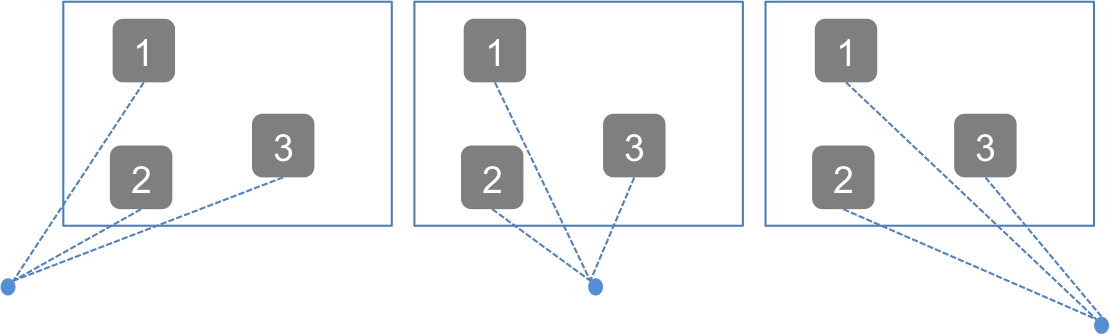
\includegraphics[width=1\columnwidth]{figures/third_principle.png}
\caption{This illustrates that when the change of user's absolution position doesn't change the relative relationship of physical targets.}
\label{fig:third_principle}
\end{figure}

\begin{figure}[t]
\centering
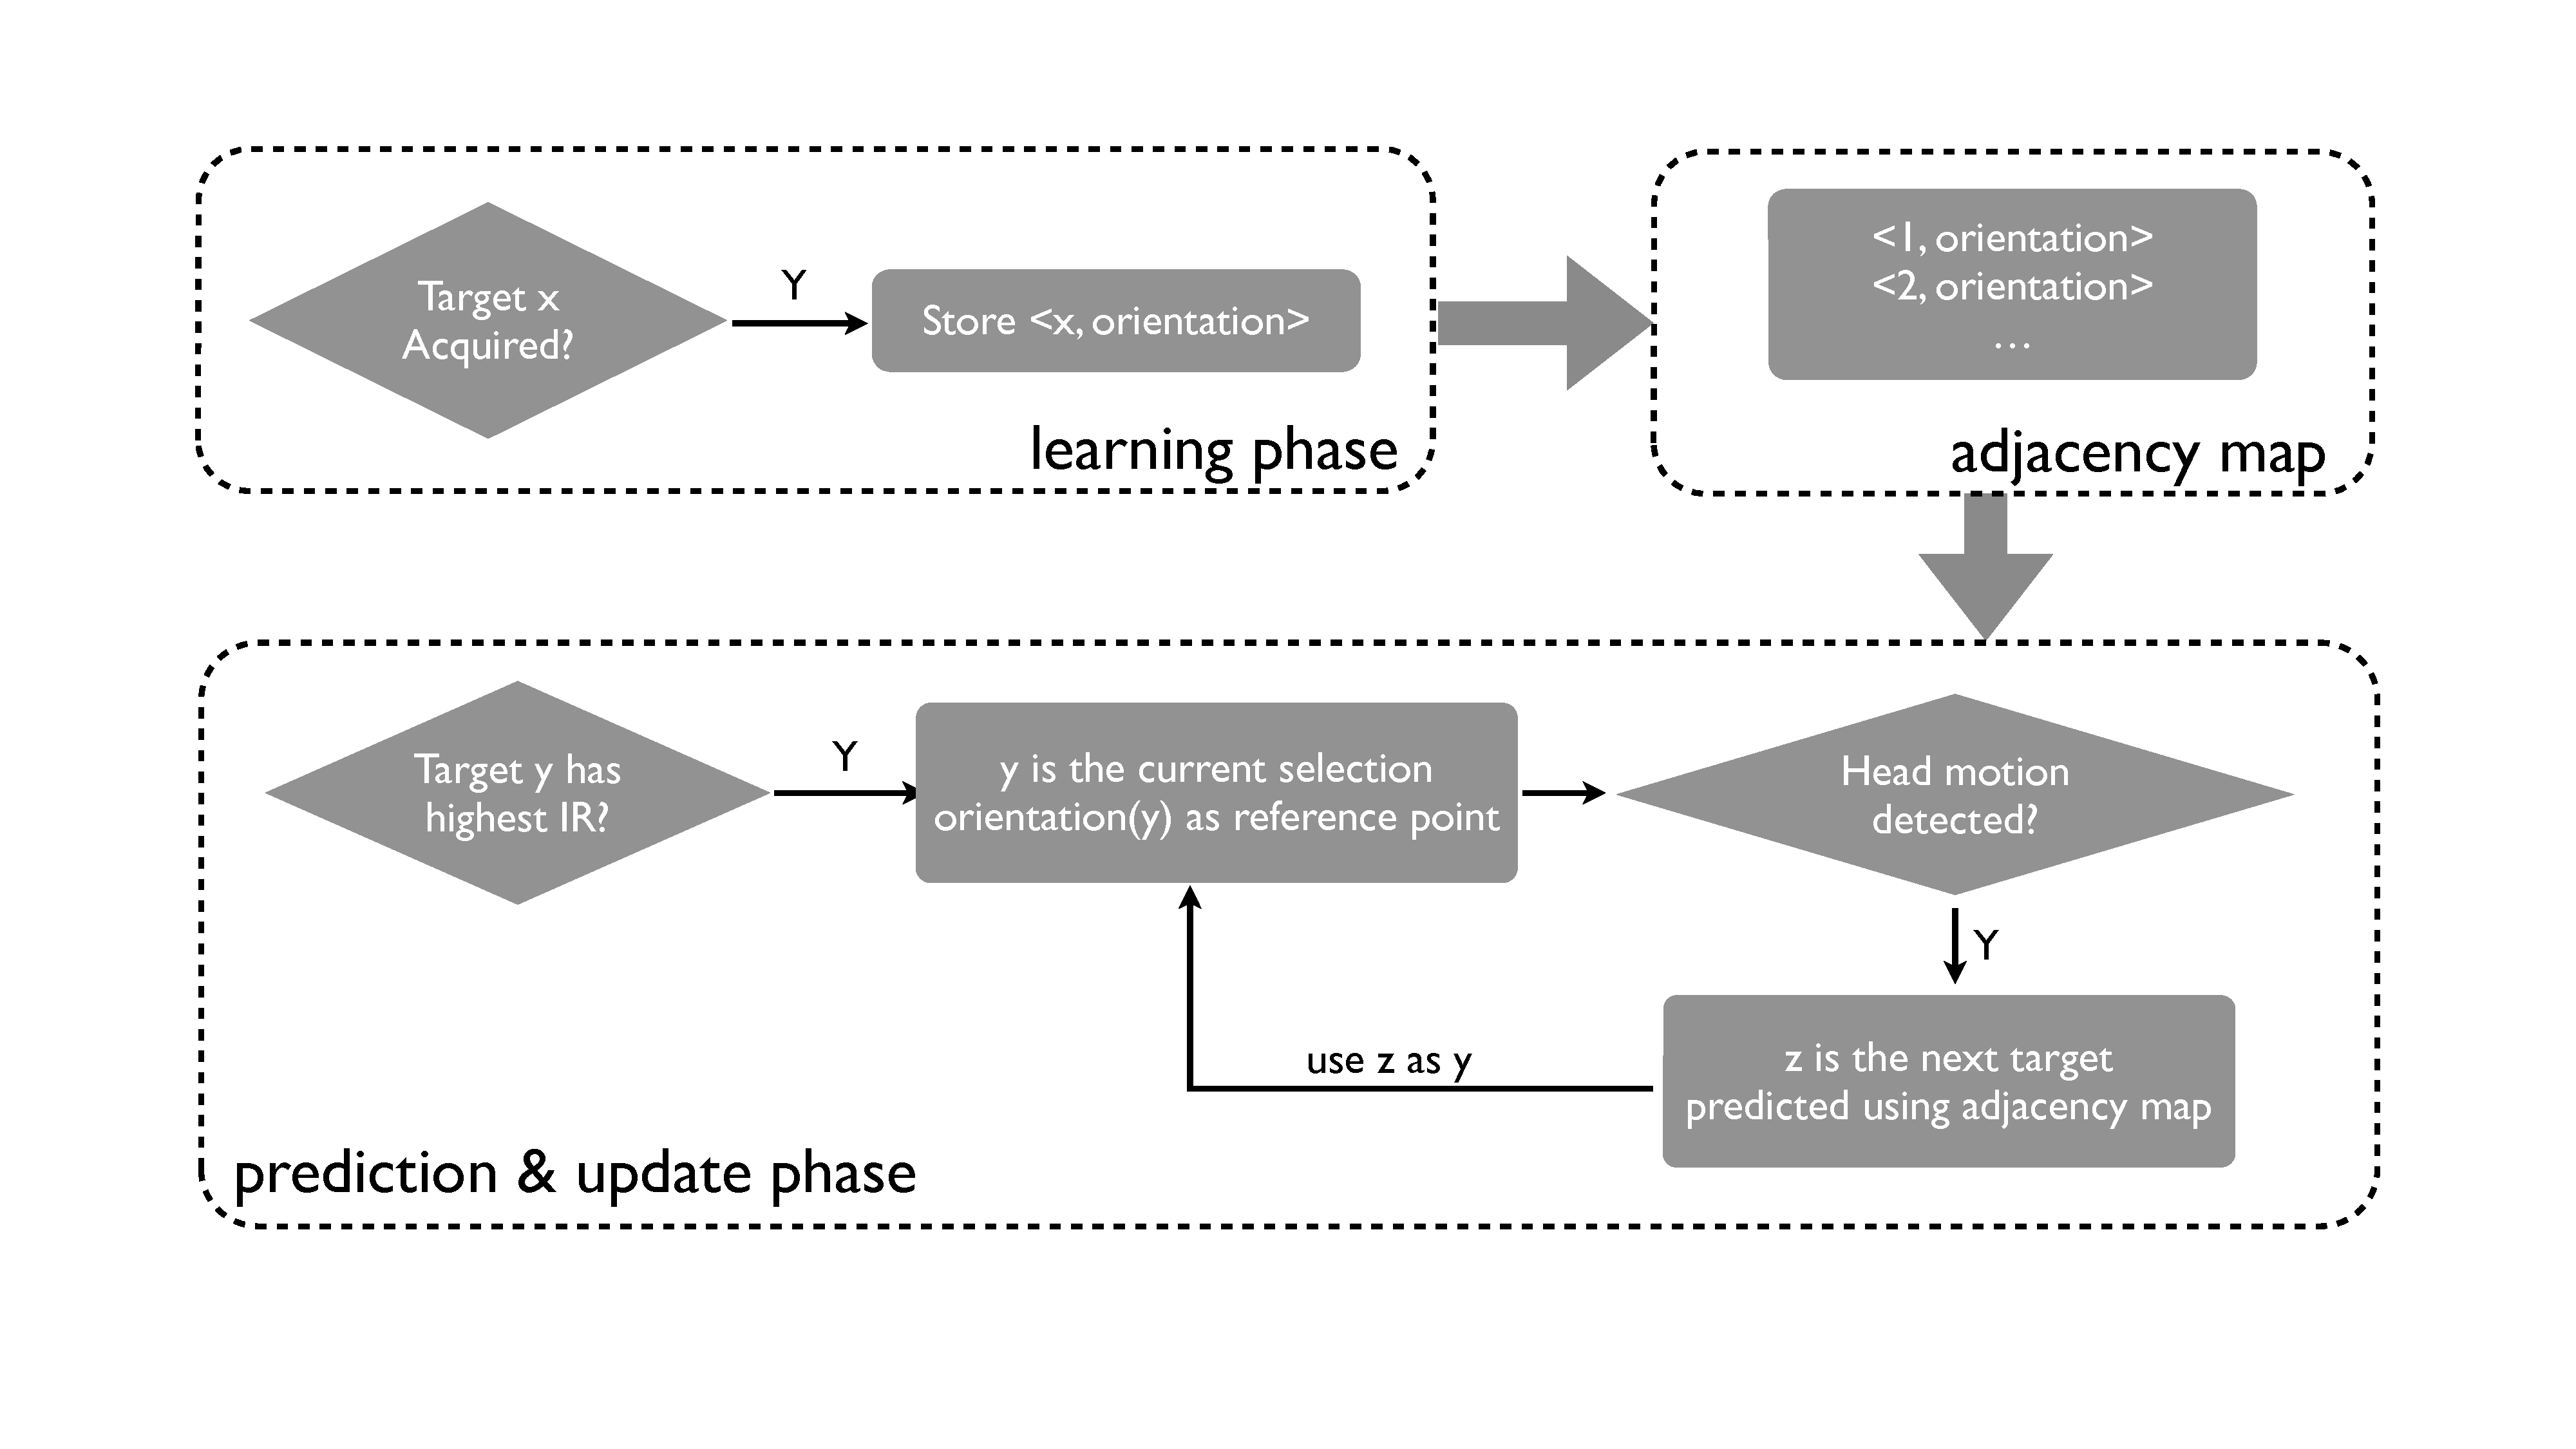
\includegraphics[width=1\columnwidth]{figures/third_technique.pdf}
\caption{Our third technique learned each target's absolute orientation and construct the adjacency map. During the {\em refinement} stage, the prediction is based on relative changes to a reference point.}
\label{fig:third_technique}
\end{figure}

After the map is created, the user can hold down on the touchpad to enter a
quasi-mode for refinement. In this quasi-mode, one device lights up at a time. When the user turns his head in the direction of another device, the light switches to that device. Therefore, the user can move between devices one at a time with slight head movements. We implement this interaction by calculating the user's direction of motion using a low-passed history of sensor measurements and searching through the adjacency map for
the nearest device in that direction. 

\subsection{Evaluation}
We evaluate the head motion refinement method by holding an informal study and collecting qualitative feedback from a subset of 4 users from the Iteration 2 study. In the study, we asked users to try cycling through the targets using the new quasi-mode.

The users had strong preferences for the new method of refinement. On a scale from 1-7, 1 being the least mental effort and 7 being the most mental effort users rated the old technique 4.25 and the new technique 2 on average. 100\% indicated a preference for head movement to list navigation. One user referenced the issue of naming targets that the list necessitates, preferring the experience of \studyquote{matching visual cues rather than numbers}. Another participant remarked that it \studyquote{just made more sense} and was a \studyquote{more natural way for demonstrating intentionality}. The users preferred the new mapping in relation to the whole environment: \studyquote{it leveraged the spatial sense that I already had just by using the system}. They were also delighted to avoid list navigation, which they now called \studyquote{difficult} and \studyquote{painful}.
